%%%%%%%%%%%%%%%%%%%%%%%%%%%%%%%%%%%%%%%%%%%%%%%%%%%%%%%%
% Este é um documento que servirá de modelo para
% os relatórios feitos na disciplina Circuitos Digitais
% 2016-2
%%%%%%%%%%%%%%%%%%%%%%%%%%%%%%%%%%%%%%%%%%%%%%%%%%%%%%%%%

\PassOptionsToPackage{brazil,american}{babel}
\documentclass[12pt]{article}

\usepackage{sbc-template}
\usepackage[brazil,american]{babel}
\usepackage[utf8]{inputenc}

\usepackage{graphicx}
\usepackage{url}
\usepackage{float}
\usepackage{listings}
\usepackage{color}
\usepackage{todonotes}
\usepackage{algorithmic}
\usepackage{algorithm}
\usepackage{hyperref}
     
\sloppy

\title{Experimento 7\\ 
Circuitos Combinacionais: Multiplexadores}

\author{Aluno 1, 10/0012345\\
        Aluno 2,  12/0123456\\
        Aluno 3, 11/1029881
}


\address{Dep. Ciência da Computação -- Universidade de Brasília (UnB)\\
  CiC 116351 - Circuitos Digitais - Turma A
  \email{\{aluno1,aluno2\}@gmail.com, aluno3@hotmail.com}
}

\begin{document} 

\maketitle

 \begin{abstract}
   Write here a short summary of the report in English. This corresponds to the Experiment 7 report on combinational circuits, specifically the multiplexers.
 \end{abstract}
     
 \begin{resumo} 
  Escreva aqui um pequeno resumo do relatório. Este corresponde ao relatório do Experimento 7 sobre circuitos combinacionais, especificamente os multiplexadores.
 \end{resumo}


\section{Objetivos}
\label{sec:Objetivos}

Descrever aqui os objetivos do experimento.

\section{Materiais} 
\label{sec:Materiais}

\begin{itemize}
    \item Painel Digital
    
    \item \textit{protoboard}
    
    \item Fios
    
    \item Portas Lógicas AND e NAND
    
\end{itemize}


\section{Introdução}
\label{sec:Introducao}

Escreva com suas palavras o que vai ser trabalhado no experimento. Aqui temos um exemplo de como citar a bibliografia consultada \cite{boulic:91} \cite{smith:99}.

\section{Procedimentos}
\label{sec:Procedimentos}

Escreva nesta seção os diversos itens pedidos no experimentos. 

\subsection{Multiplexador de 4 entradas}
\label{sec:Mux}

Descrever o experimento realizado. Sempre  que colocar uma figura deve-se explicar o que se pretende que o leitor veja, ou uma análise logo após a figura. 

\begin{figure}[H]
\centering
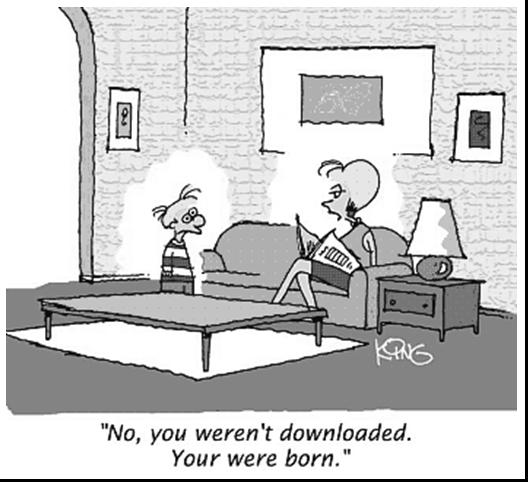
\includegraphics[width=.5\textwidth]{fig1.jpg}
\caption{Uma figura}
\label{fig:exemplo}
\end{figure}

A Figura~\ref{fig:exemplo} apresenta um exemplo de como usar e citar uma figura.

Aqui temos um exemplo de como citar uma URL na bibliografia~\cite{systemverilog}.
Aqui temos um exemplo de como criar um hiperlink. Veja
\href{https://www.youtube.com/watch?v=EcNxjxKRQ6E}{aqui} um exemplo de vídeo.

Sempre identifique no site do vídeo:
\begin{itemize}
    \item o experimento: Experimento 7;
    \item semestre: 2016-2;
    \item a disciplina: CiC 116351 - Circuitos Digitais - Turma B;
    \item a universidade: Universidade de Brasília (UnB);
    \item os nomes dos componentes do grupo.
\end{itemize}

É apresentado acima como fazer uma listagem não numerada.

\subsection{Demultiplexador}
\label{sec:Demux}

Este é outro item do experimento.
Aqui temos um exemplo de como construir e citar uma tabela, conforme mostrado na Tabela~\ref{tab:resultados}.

\begin{table}[H]
    \centering
    \caption{Expected values of the obtained circuits' attributes.}
    \begin{tabular}{|c|c|c|c|c|c|c|c|}
    \cline{2-7}
    \multicolumn{1}{c}{} & \multicolumn{3}{|c|}{Phase 1} & \multicolumn{3}{c|}{Phase 2} & \multicolumn{1}{c}{} \\
    \hline
    Experiment & $n_g$ & $n_l$ & $n_t$ & $n_g$ & $n_l$ & $n_t$ & $t(s)$ \\
    \hline
    1 bit full adder & 8.16 & 3.8 & 47.6 & 5.03 & 3.0 & 25.93 & 99.13 \\
    2 bit full adder & 18.06 & 5.16 & 107.13 & 11.06 & 4.9 & 60.06 & 709.56 \\
    2 bit multiplier & 14.2 & 4.03 & 74.33 & 7.7 & 2.2 & 37.53 & 357.76 \\
    7 segment decoder & 47.53 & 5.83 & 270.46 & 32.86 & 5.0 & 176.4 & 740.63 \\
    Karnaugh 1 bit full adder & 19.0 & 6.0 & 102.0 & 5.03 & 3.0 & 24.8 & 130.73 \\
    \hline
    \end{tabular}
    \label{tab:resultados}
\end{table}

Aqui devemos colocar uma apresentação e análise da tabela, explicando ao leitor o que se pretende mostrar.

\section{Análise dos Resultados}
\label{sec:Resultados}

Faça uma análise crítica dos resultados obtidos nos experimentos. Esta análise pode ser feita item a item ou de uma forma geral.

Dica: Use pesquisa na Internet para tirar as dúvidas sobre edição em \LaTeX .

\section{Conclusão}
\label{sec:Conclusao}

Concluir o relatório explanando rapidamente o que foi feito e os resultados obtidos, sempre correlacionando com os objetivos do experimento apresentado na Seção~\ref{sec:Objetivos}. 


\bibliographystyle{sbc}
\bibliography{relatorio}


\newpage 
% Colocar aqui apenas as respostas dos itens da Auto-Avaliação
\section*{Auto-Avaliação}

\begin{enumerate}
    \item a
    \item c
    \item b
    \item d
\end{enumerate}


\end{document}
